\documentclass[12pt]{article}
\usepackage[a4paper, bindingoffset=0.2in, %
							left=0.5in,right=0.5in,top=0.5in,bottom=0.5in,%
							footskip=.25in]{geometry}
\usepackage{graphicx}
\usepackage{listings}
\usepackage{amssymb}
\usepackage{amsmath}
\usepackage{hyperref}


\title{PSet3 Report}
\author{Ali Abolhassanzadeh Mahani}
%\date{Oct. 15}

\begin{document}
	\maketitle
	
	\section{Coloring Algorithm}
	I added a new vertical array to the left side of my grid to initialize the clusters. The algorithm is as you said
	in your class. I used numbers from 1 to ... for the cells that are \emph{on} and 0 for cells that are \emph{off}.
	Now you can see the picture in Fig \ref{fig:Color}
	\begin{figure}[h!]
		\centering
		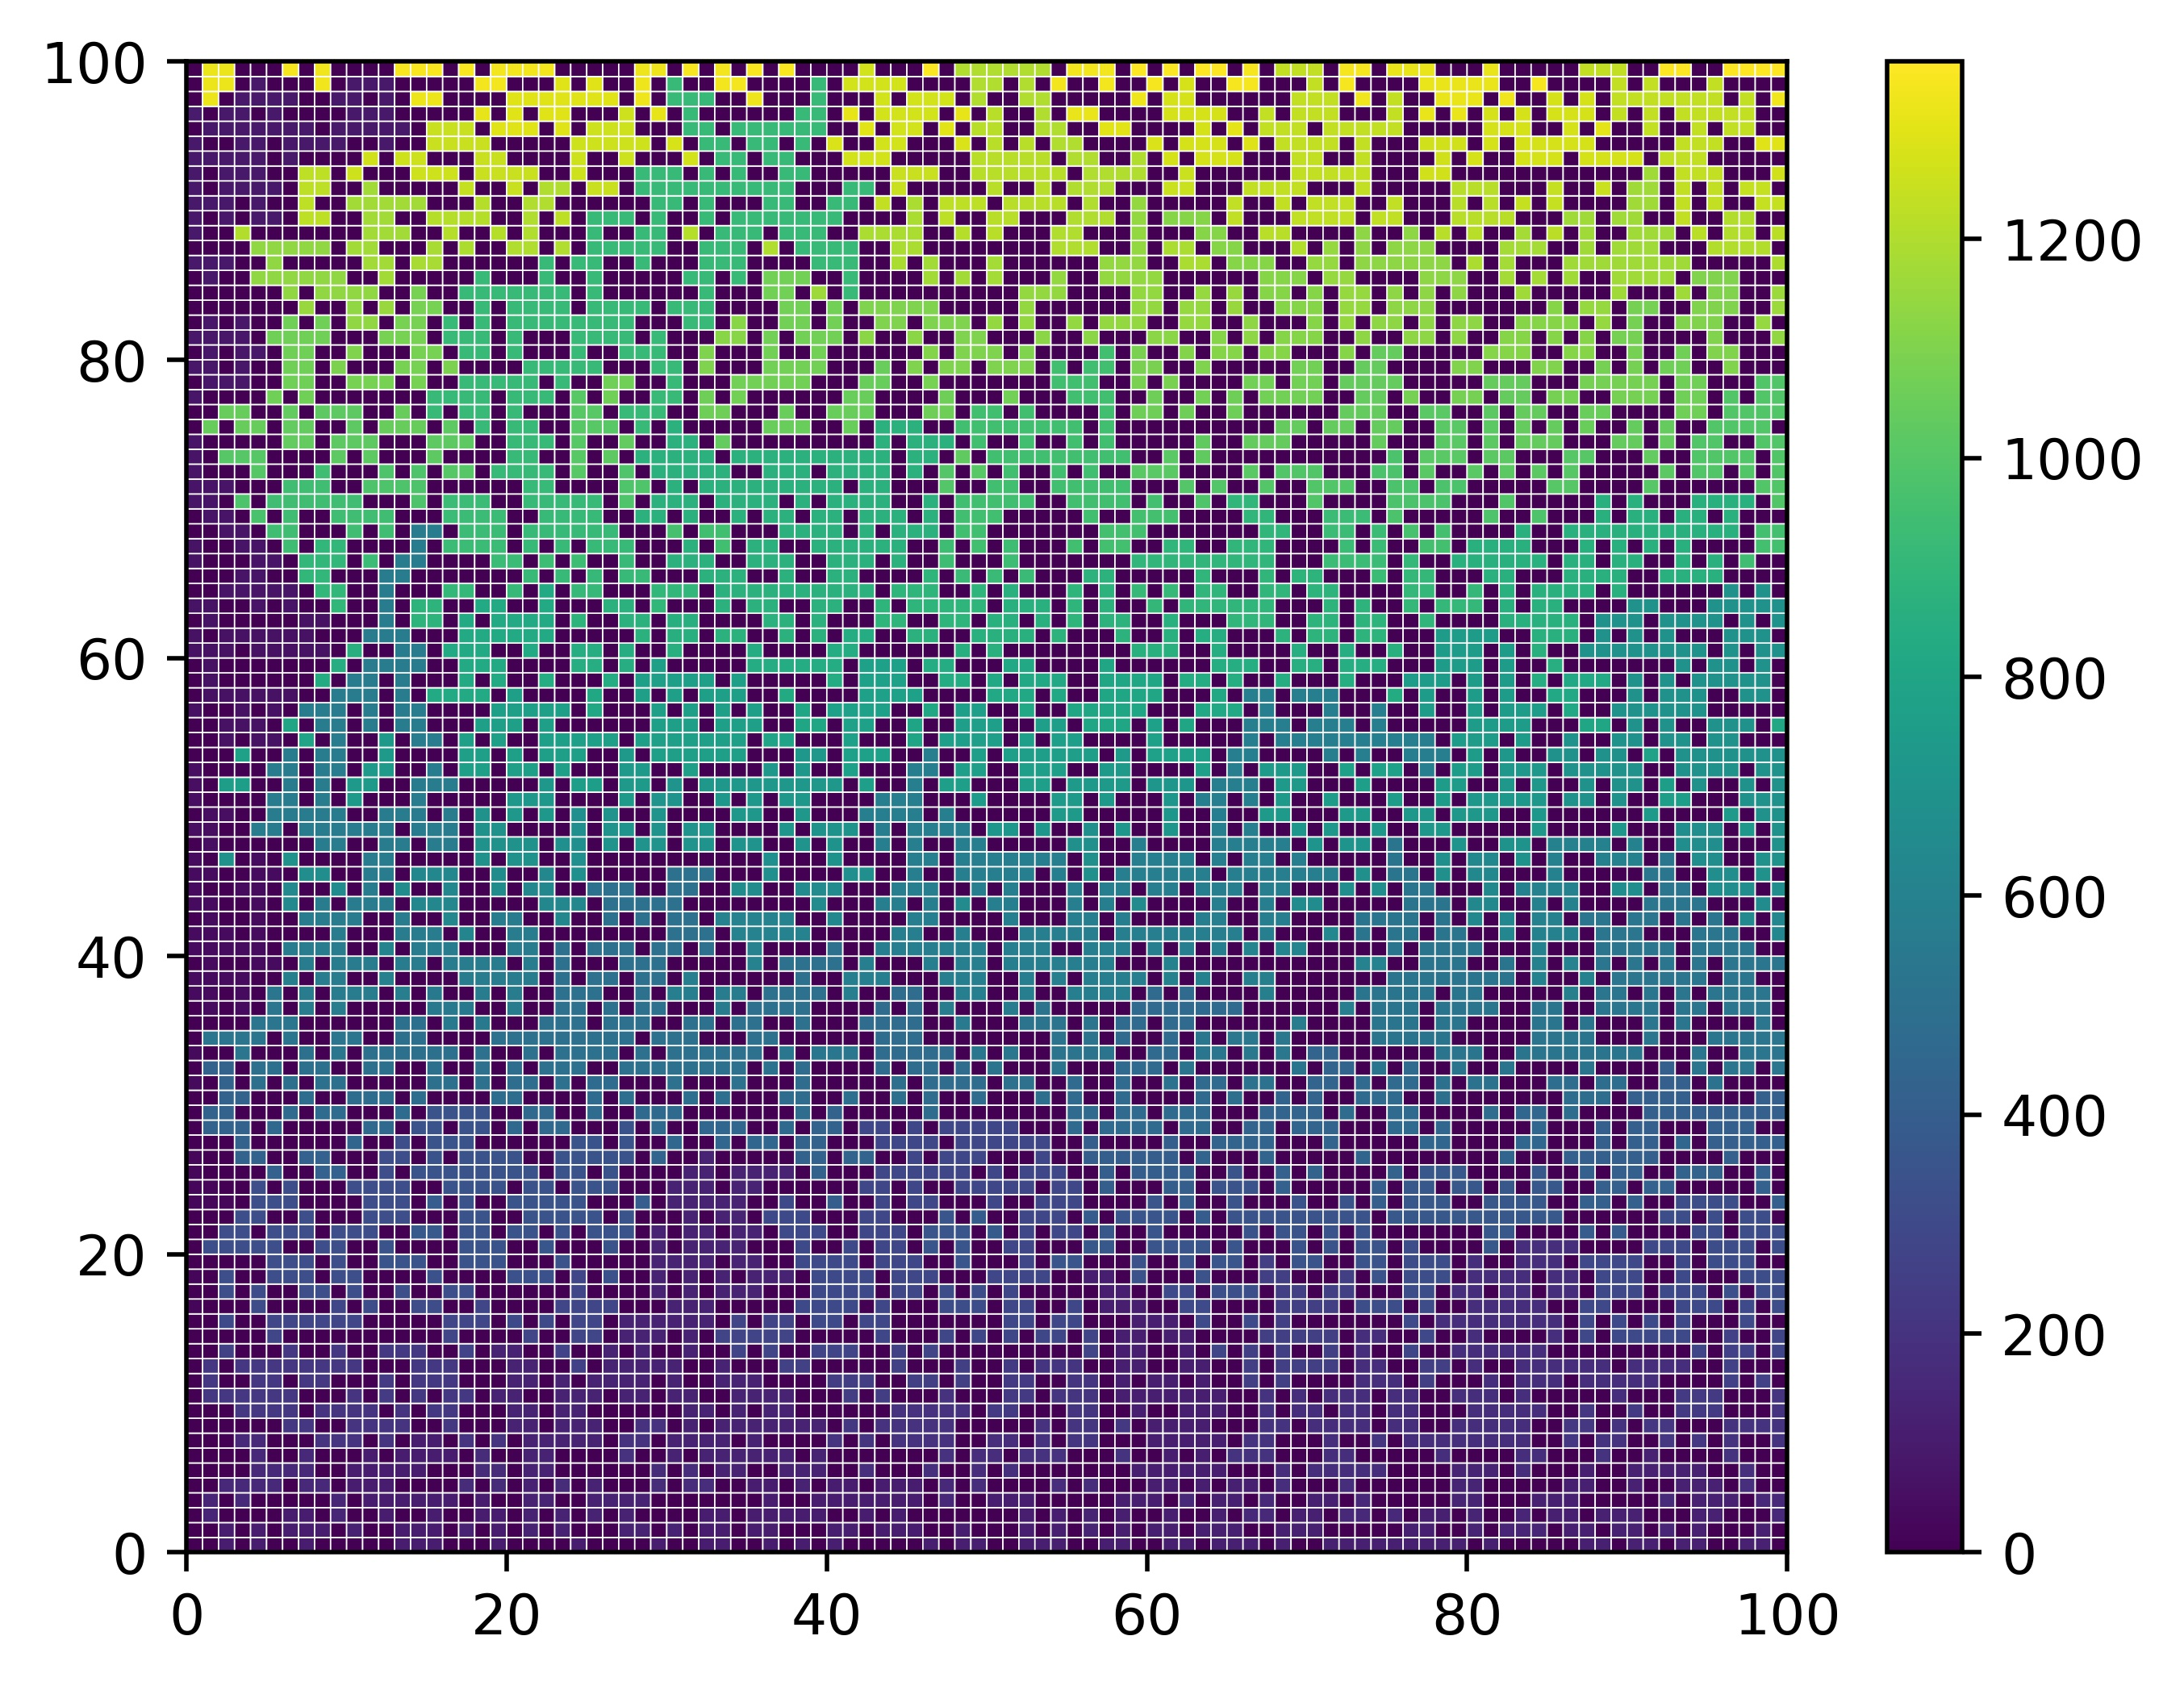
\includegraphics[width=0.9\linewidth]{../p2/colored.jpg}
		\label{fig:Color}
		\caption{Simulation of horizontal percolation for a 100 * 100 grid with probability 0.5. The cells with number 0 are \emph{off} and the ones with the same color form a \emph{clutser}}
	\end{figure}
	
	\section{Probability of Percolation (Question 3)}
	I used the coloring algorithm with pointers to find clusters and then a method called \texttt{is\_percolated(grid)} that takes the grid and loops over the last
	row to see if any of the items have a number in the range of the length of our grid. This is the definition of percolation due to the details of
	our clustering and coloring code specified in the previous section. The runtime complexity is of order $\mathcal{O}(L^2)$ with $L$ being the 
	size of a row.
	I plotted all the data in on plot available in Fig\ref{fig:Perc}
	\begin{figure}[h!]
		\centering
		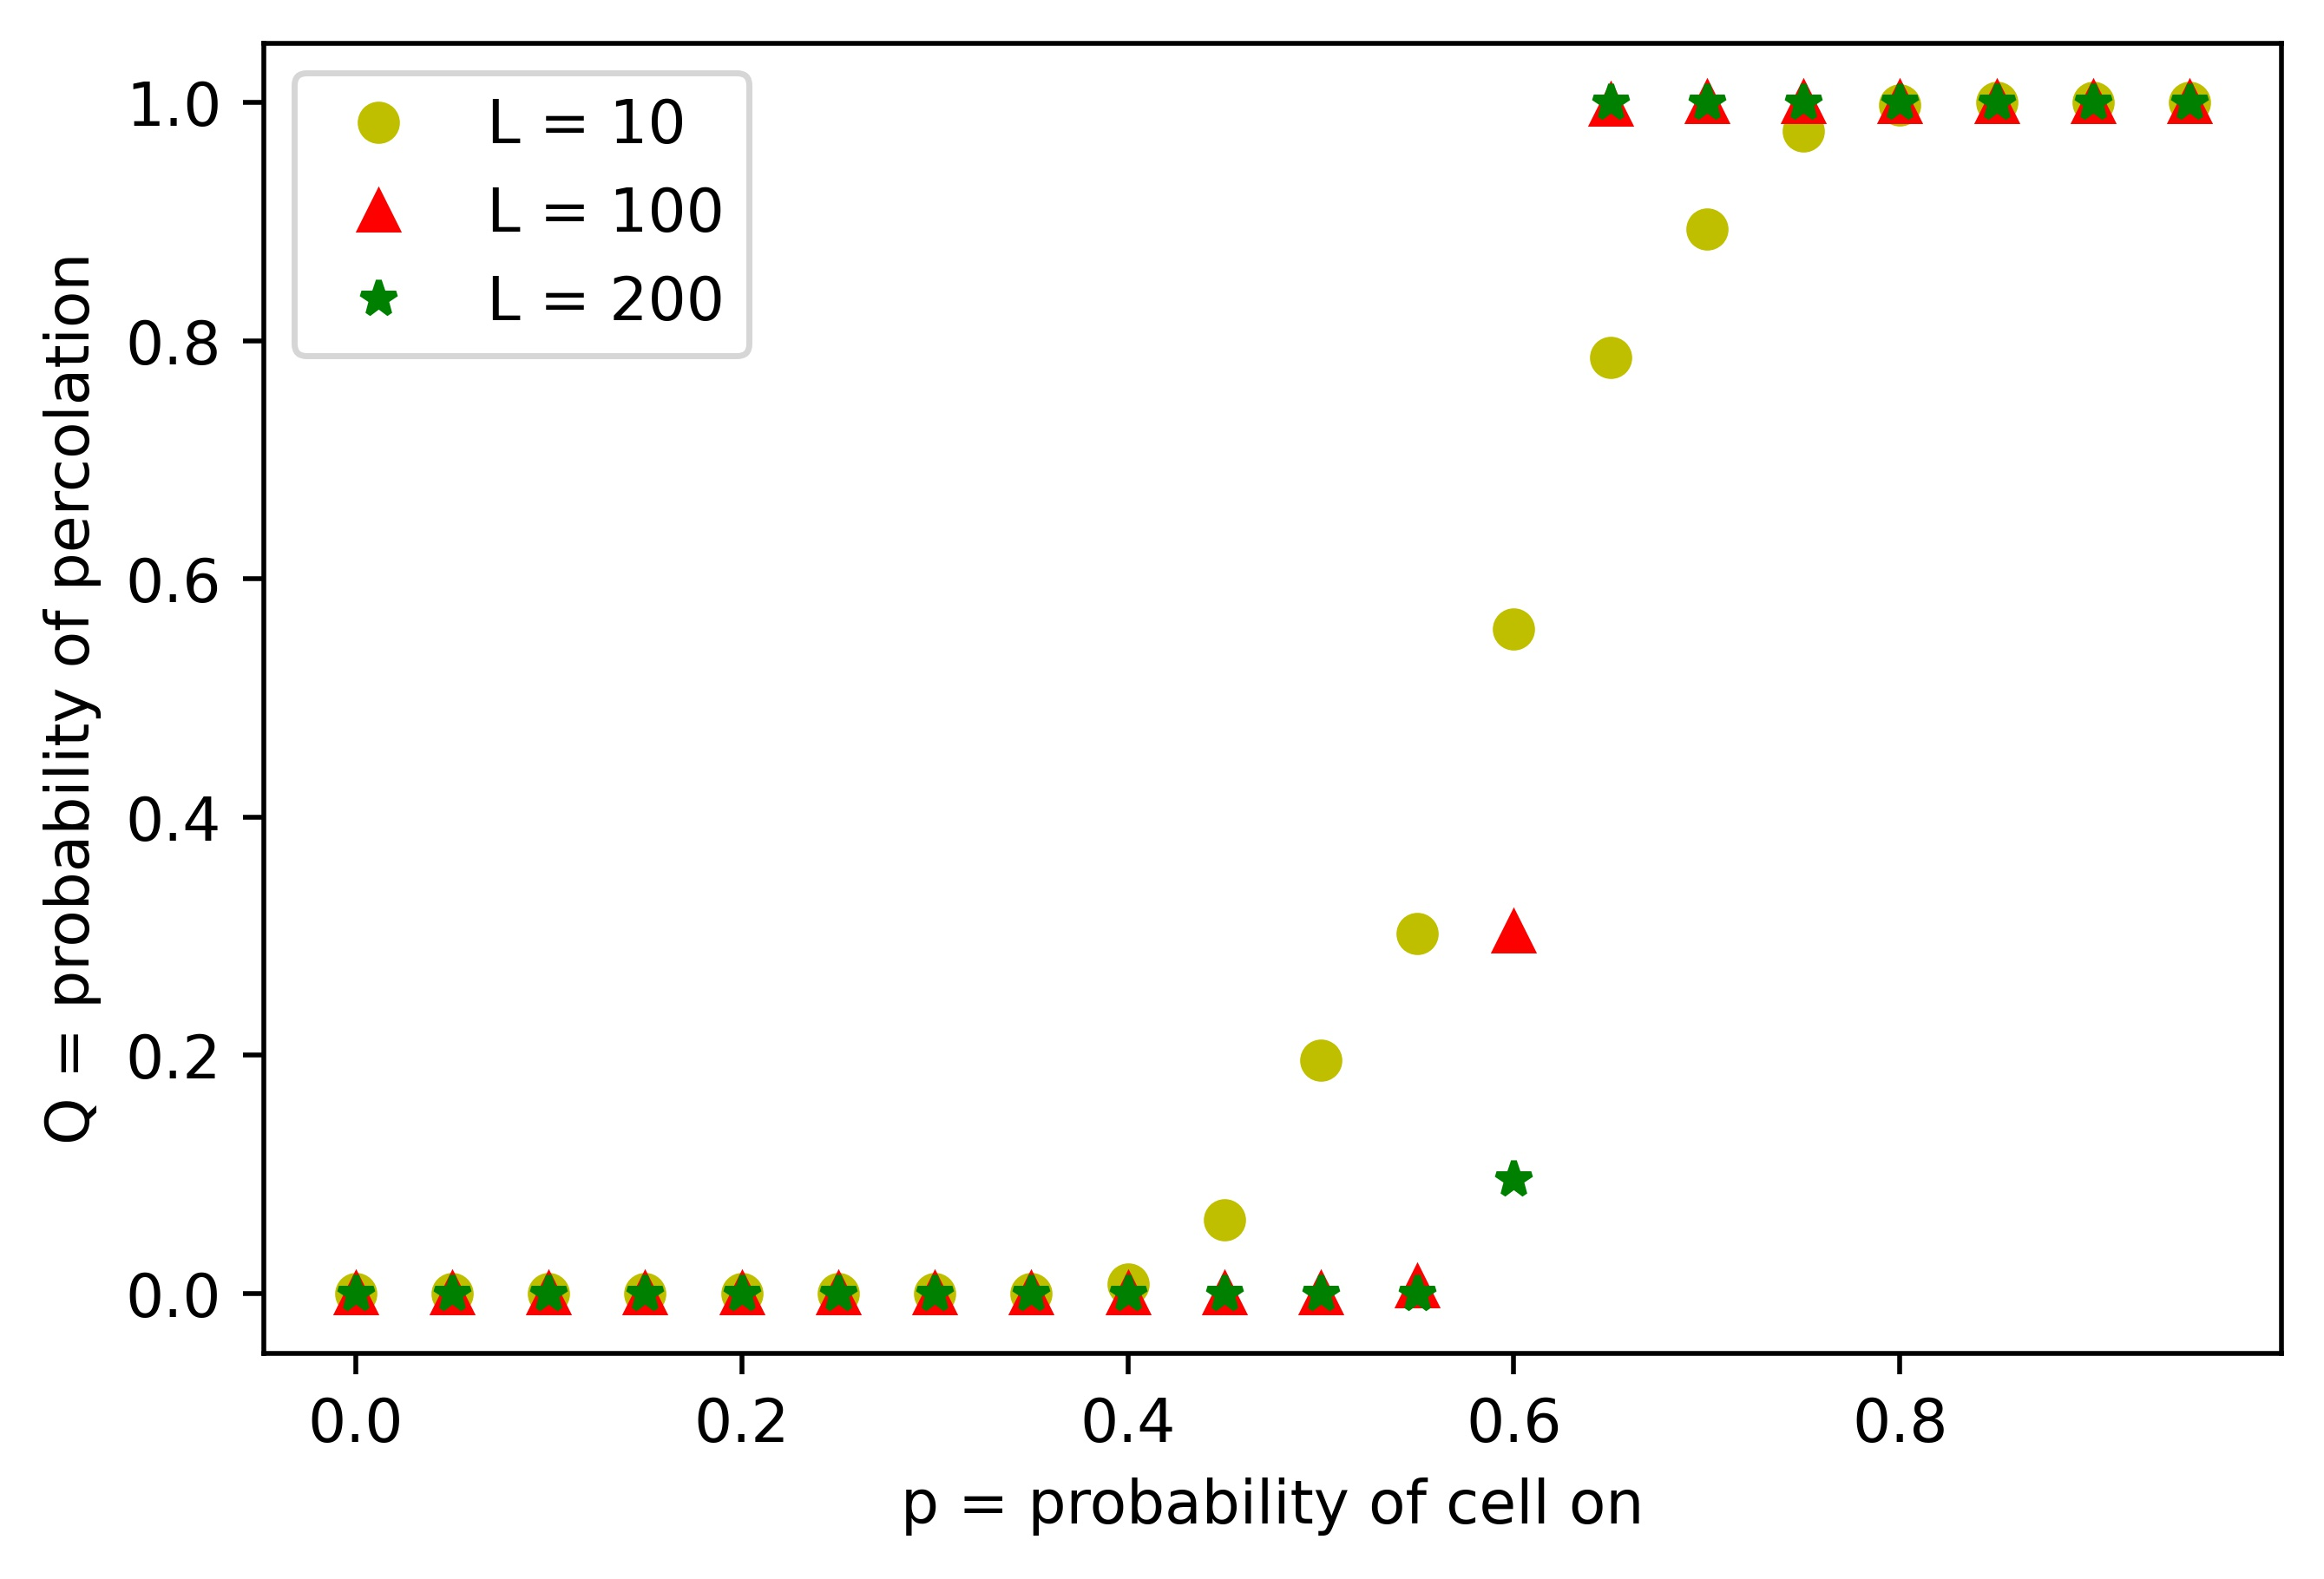
\includegraphics[width=0.9\linewidth]{../p3/percs.jpg}
		\label{fig:Perc}
		\caption{Plot for $Q$ vs. $p$ for matrix side lengths $L = 10, 100, 200$.}
	\end{figure}
	
	\section{Probability of being attached to the infinite cluster $Q_\infty$}
	I changed the \texttt{is\_percolated()} function to store the color code of the percolating cluster. Then I 
	loop over the the matrix again and find $Q_\infty$. I loop for 100 runs for each $p$ and take the mean.\\
	The plot is available in Fig\ref{fig:percProb}
	\begin{figure}[h!]
		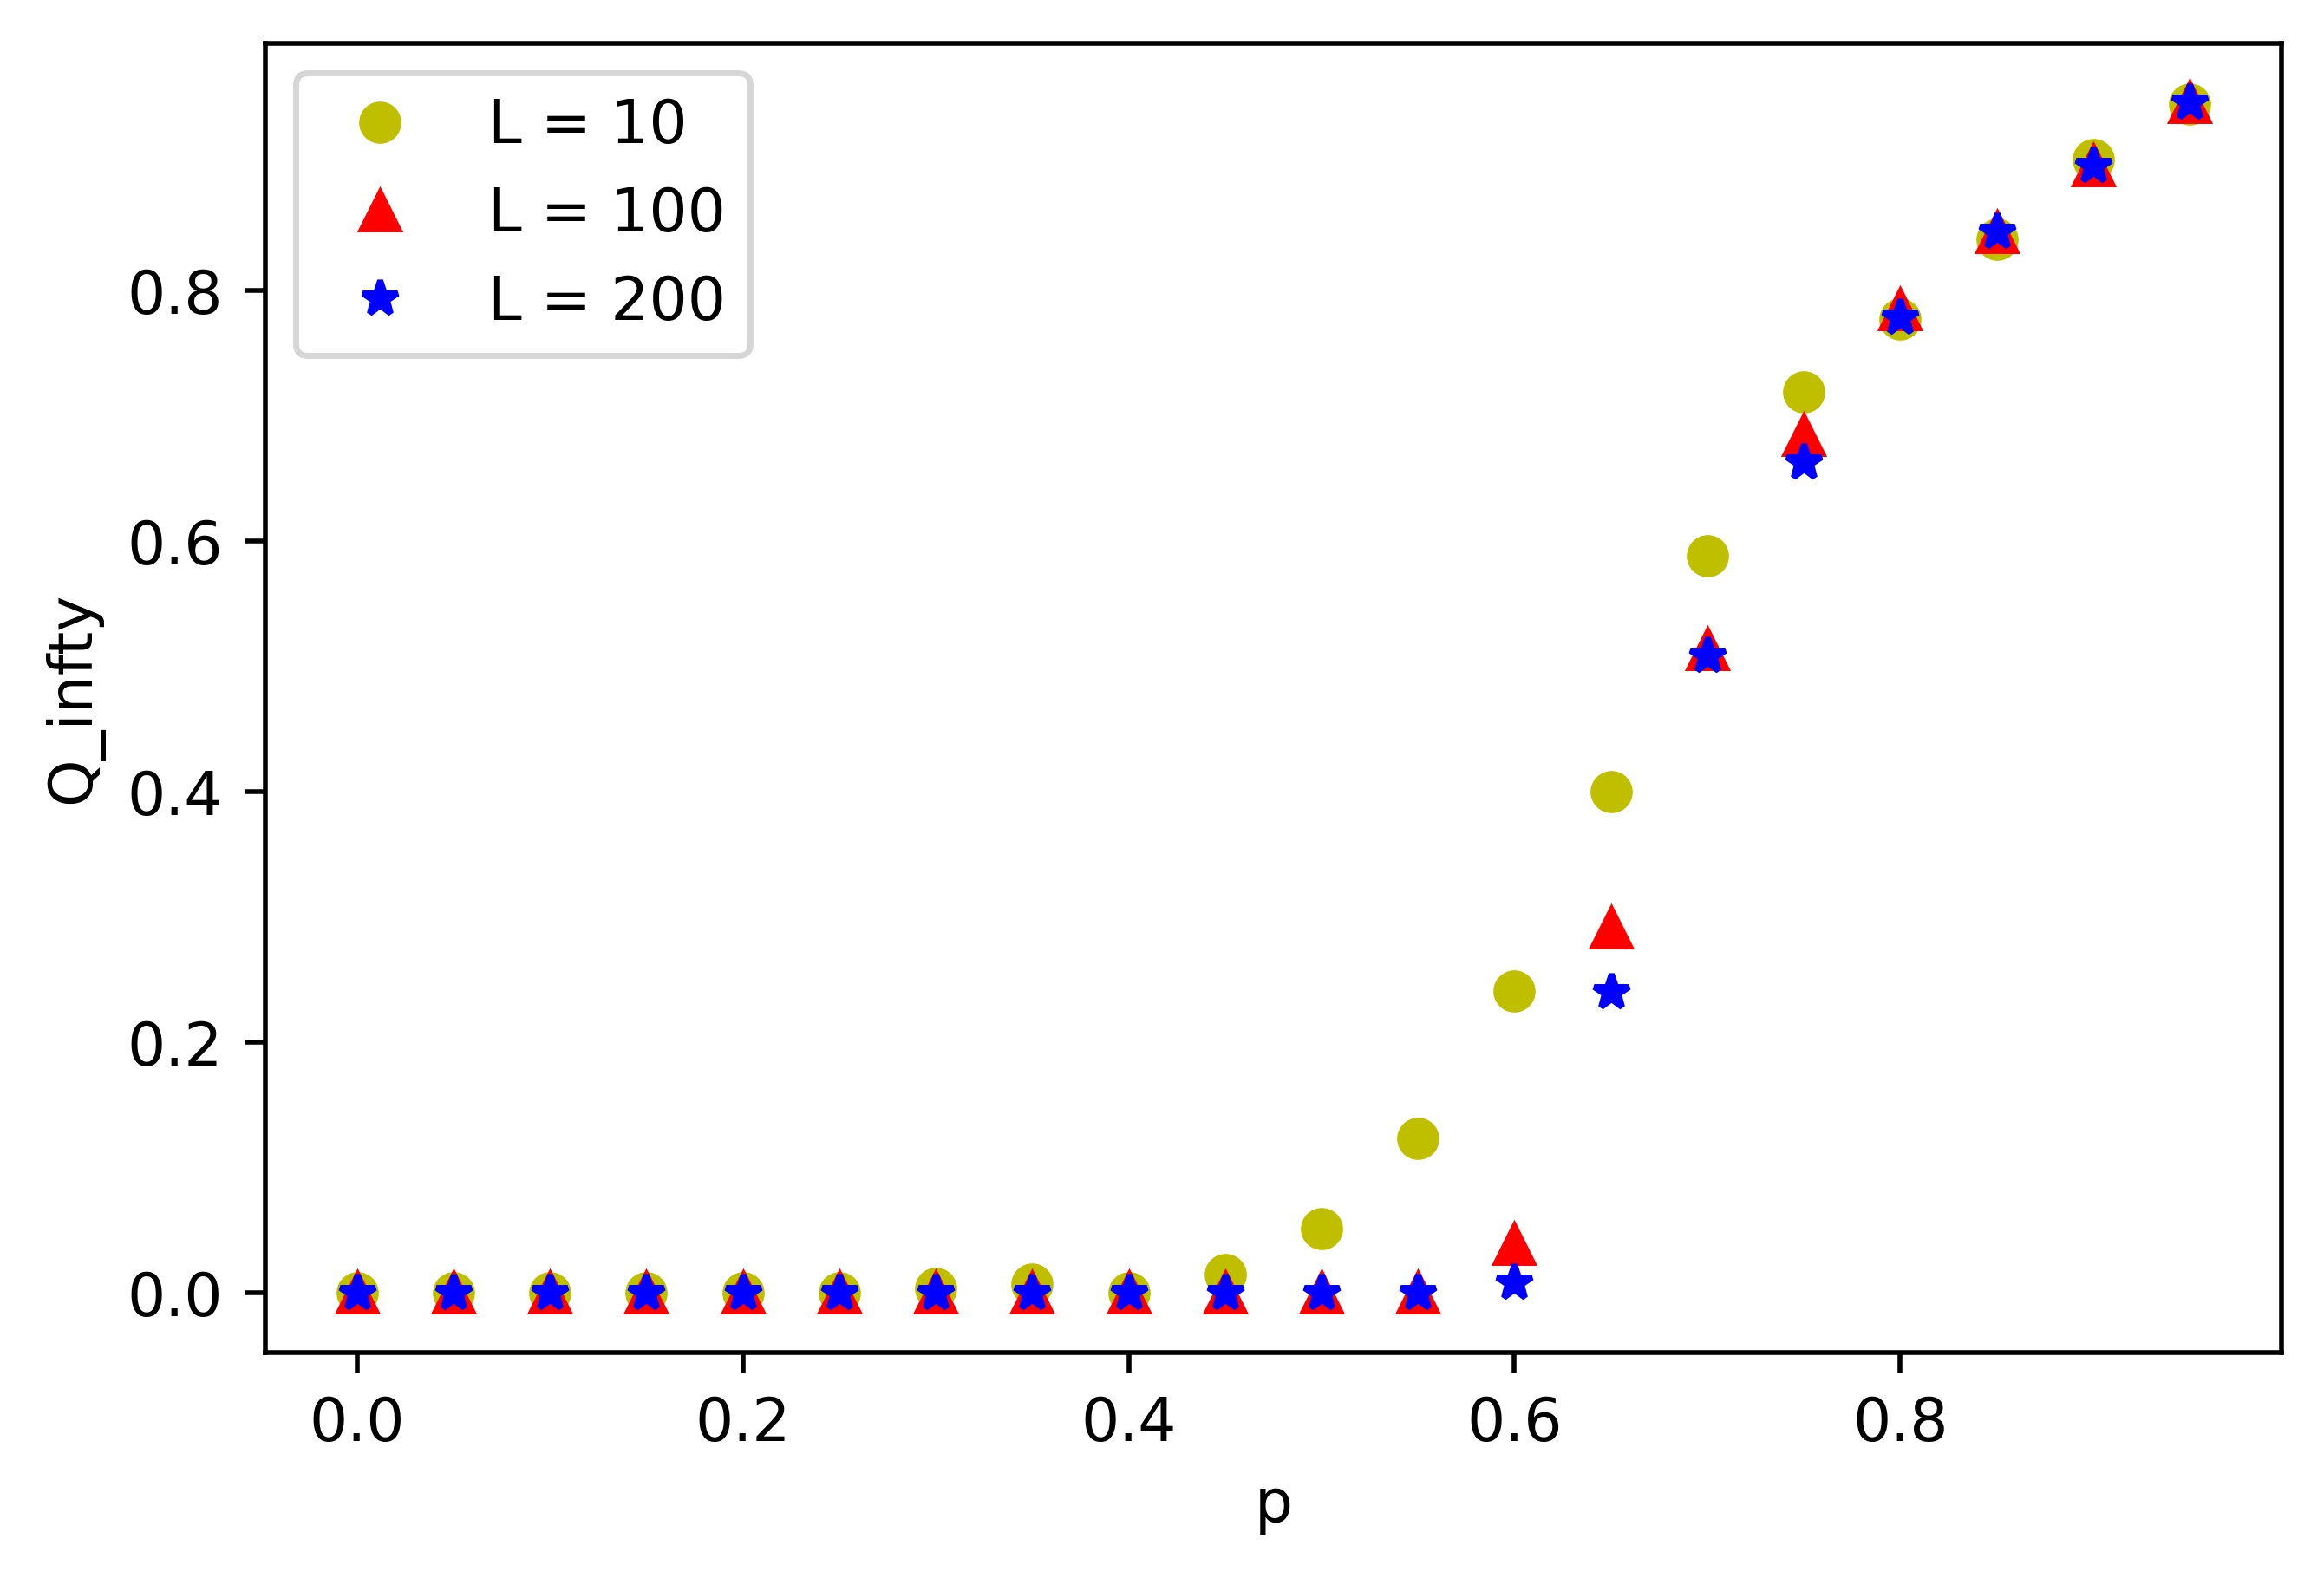
\includegraphics[width=0.9\linewidth]{../p4/percProb.jpg}
		\label{fig:percProb}
		\caption{\emph{Percolation Probability $Q_\infty$} vs \emph{$p$} for p from 0 to 0.95}
	\end{figure}
	
	\section{Gyro Radius of the greatest non-infinite cluster}
	I wrote a function \texttt{not\_percCluster(int color)} to rule out the colors for all the percolating clusters. Then, I wrote \texttt{findNextGyro()} to loop over the matrix, find the cluster coordinate, and then calculate the gyro radius for it.
	
	I looped for probability intervals of 0.025 and plotted the results for lengths $L = \{10, 20, 40, 80, 160\}$ in 
	Fig\ref{fig:gyroCluster}. It's worth mentioning that I looped 6000 times for 10, 2000 for 20, 1000 for 40, 500 for 800 and 100 for 160.
	
	My runtime for this problem is as follows:\\
	\centerline{\texttt{Time elapsed: 1420.6 seconds}}
	\begin{figure}[h!]
		\centering
		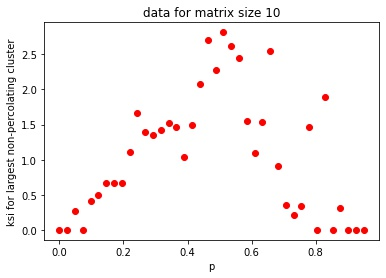
\includegraphics[width=0.9\linewidth]{../p5/fig0.jpg}
		\label{fig:gyroCluster}
		\caption{The plot for mean gyro radius  of greatest non-percolating clusters vs. probability of cell being on. For lengths $L = \{10, 20, 40, 80, 160\}$}
	\end{figure}
	\begin{figure}[h!]
	\centering
		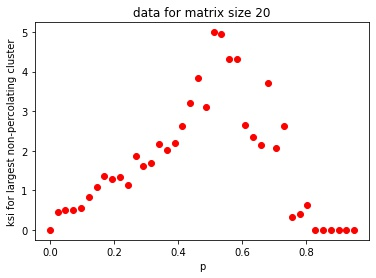
\includegraphics[width=0.9\linewidth]{../p5/fig1.jpg}
	\label{fig:gyroCluste1}
	\caption{The plot for mean gyro radius  of greatest non-percolating clusters vs. probability of cell being on. For lengths $L = \{10, 20, 40, 80, 160\}$}
\end{figure}
	\begin{figure}[h!]
	\centering
	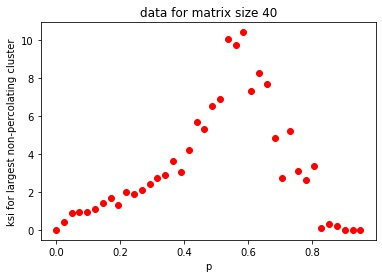
\includegraphics[width=0.9\linewidth]{../p5/fig2.jpg}
	\label{fig:gyroCluste2}
	\caption{The plot for mean gyro radius  of greatest non-percolating clusters vs. probability of cell being on. For lengths $L = \{10, 20, 40, 80, 160\}$}
\end{figure}
	\begin{figure}[h!]
	\centering
	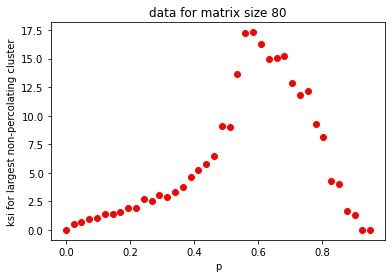
\includegraphics[width=0.9\linewidth]{../p5/fig3.jpg}
	\label{fig:gyroCluster3}
	\caption{The plot for mean gyro radius  of greatest non-percolating clusters vs. probability of cell being on. For lengths $L = \{10, 20, 40, 80, 160\}$}
\end{figure}
	\begin{figure}[h!]
	\centering
	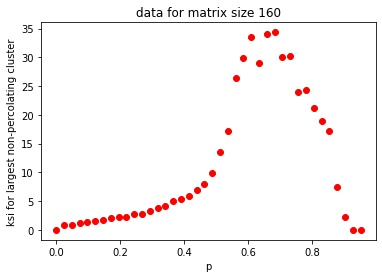
\includegraphics[width=0.9\linewidth]{../p5/fig4.jpg}
	\label{fig:gyroCluster4}
	\caption{The plot for mean gyro radius  of greatest non-percolating clusters vs. probability of cell being on. For lengths $L = \{10, 20, 40, 80, 160\}$}
\end{figure}

	\section{The critical power $\nu$}
	As we did in the previous section, we now the critical probabilities in which phase shift happens. Now we know that this probability for length $L$ is related to the infinite length (unbounded) probability with the equation below:\\
	\begin{equation}
		|p_c(L) - p_c(\infty)| \sim L^{-\frac{1}{\nu}}
	\end{equation}
	where $\nu$ is the critical power. We plot $\log_{10}(y)$ vs. $\log_{10}(L)$ and fit a line to the data to get
	the value for the slope and this way, we can find $\nu$.
	The value for the slope is as follows:\\
	\centerline{\texttt{Slope is -0.30502 (+/-) 0.65170}}\\
	and so the value for $\nu$ is:\\
	\centerline{\texttt{nu is 3.27852 (+/-) 0.65170}}\\
	The relative error percentile is $\eta = 145.88 \%$

	\section{The Mass Dimention of the Percolation Clusters (Problem 7)}
	I did the simulation 150 times for each probability. I got \texttt{segmentation fault} error for 0.59 so I reduced it to 0.588 and it worked.
	I drew the plots available in Fig\ref{fig:area-gyro}.
	I fitted the data and This is the value to the slope:\\
	\centerline{\texttt{Slope is 1.923 (+/-) 0.009}}
	\begin{figure}[h!]
		\centering
		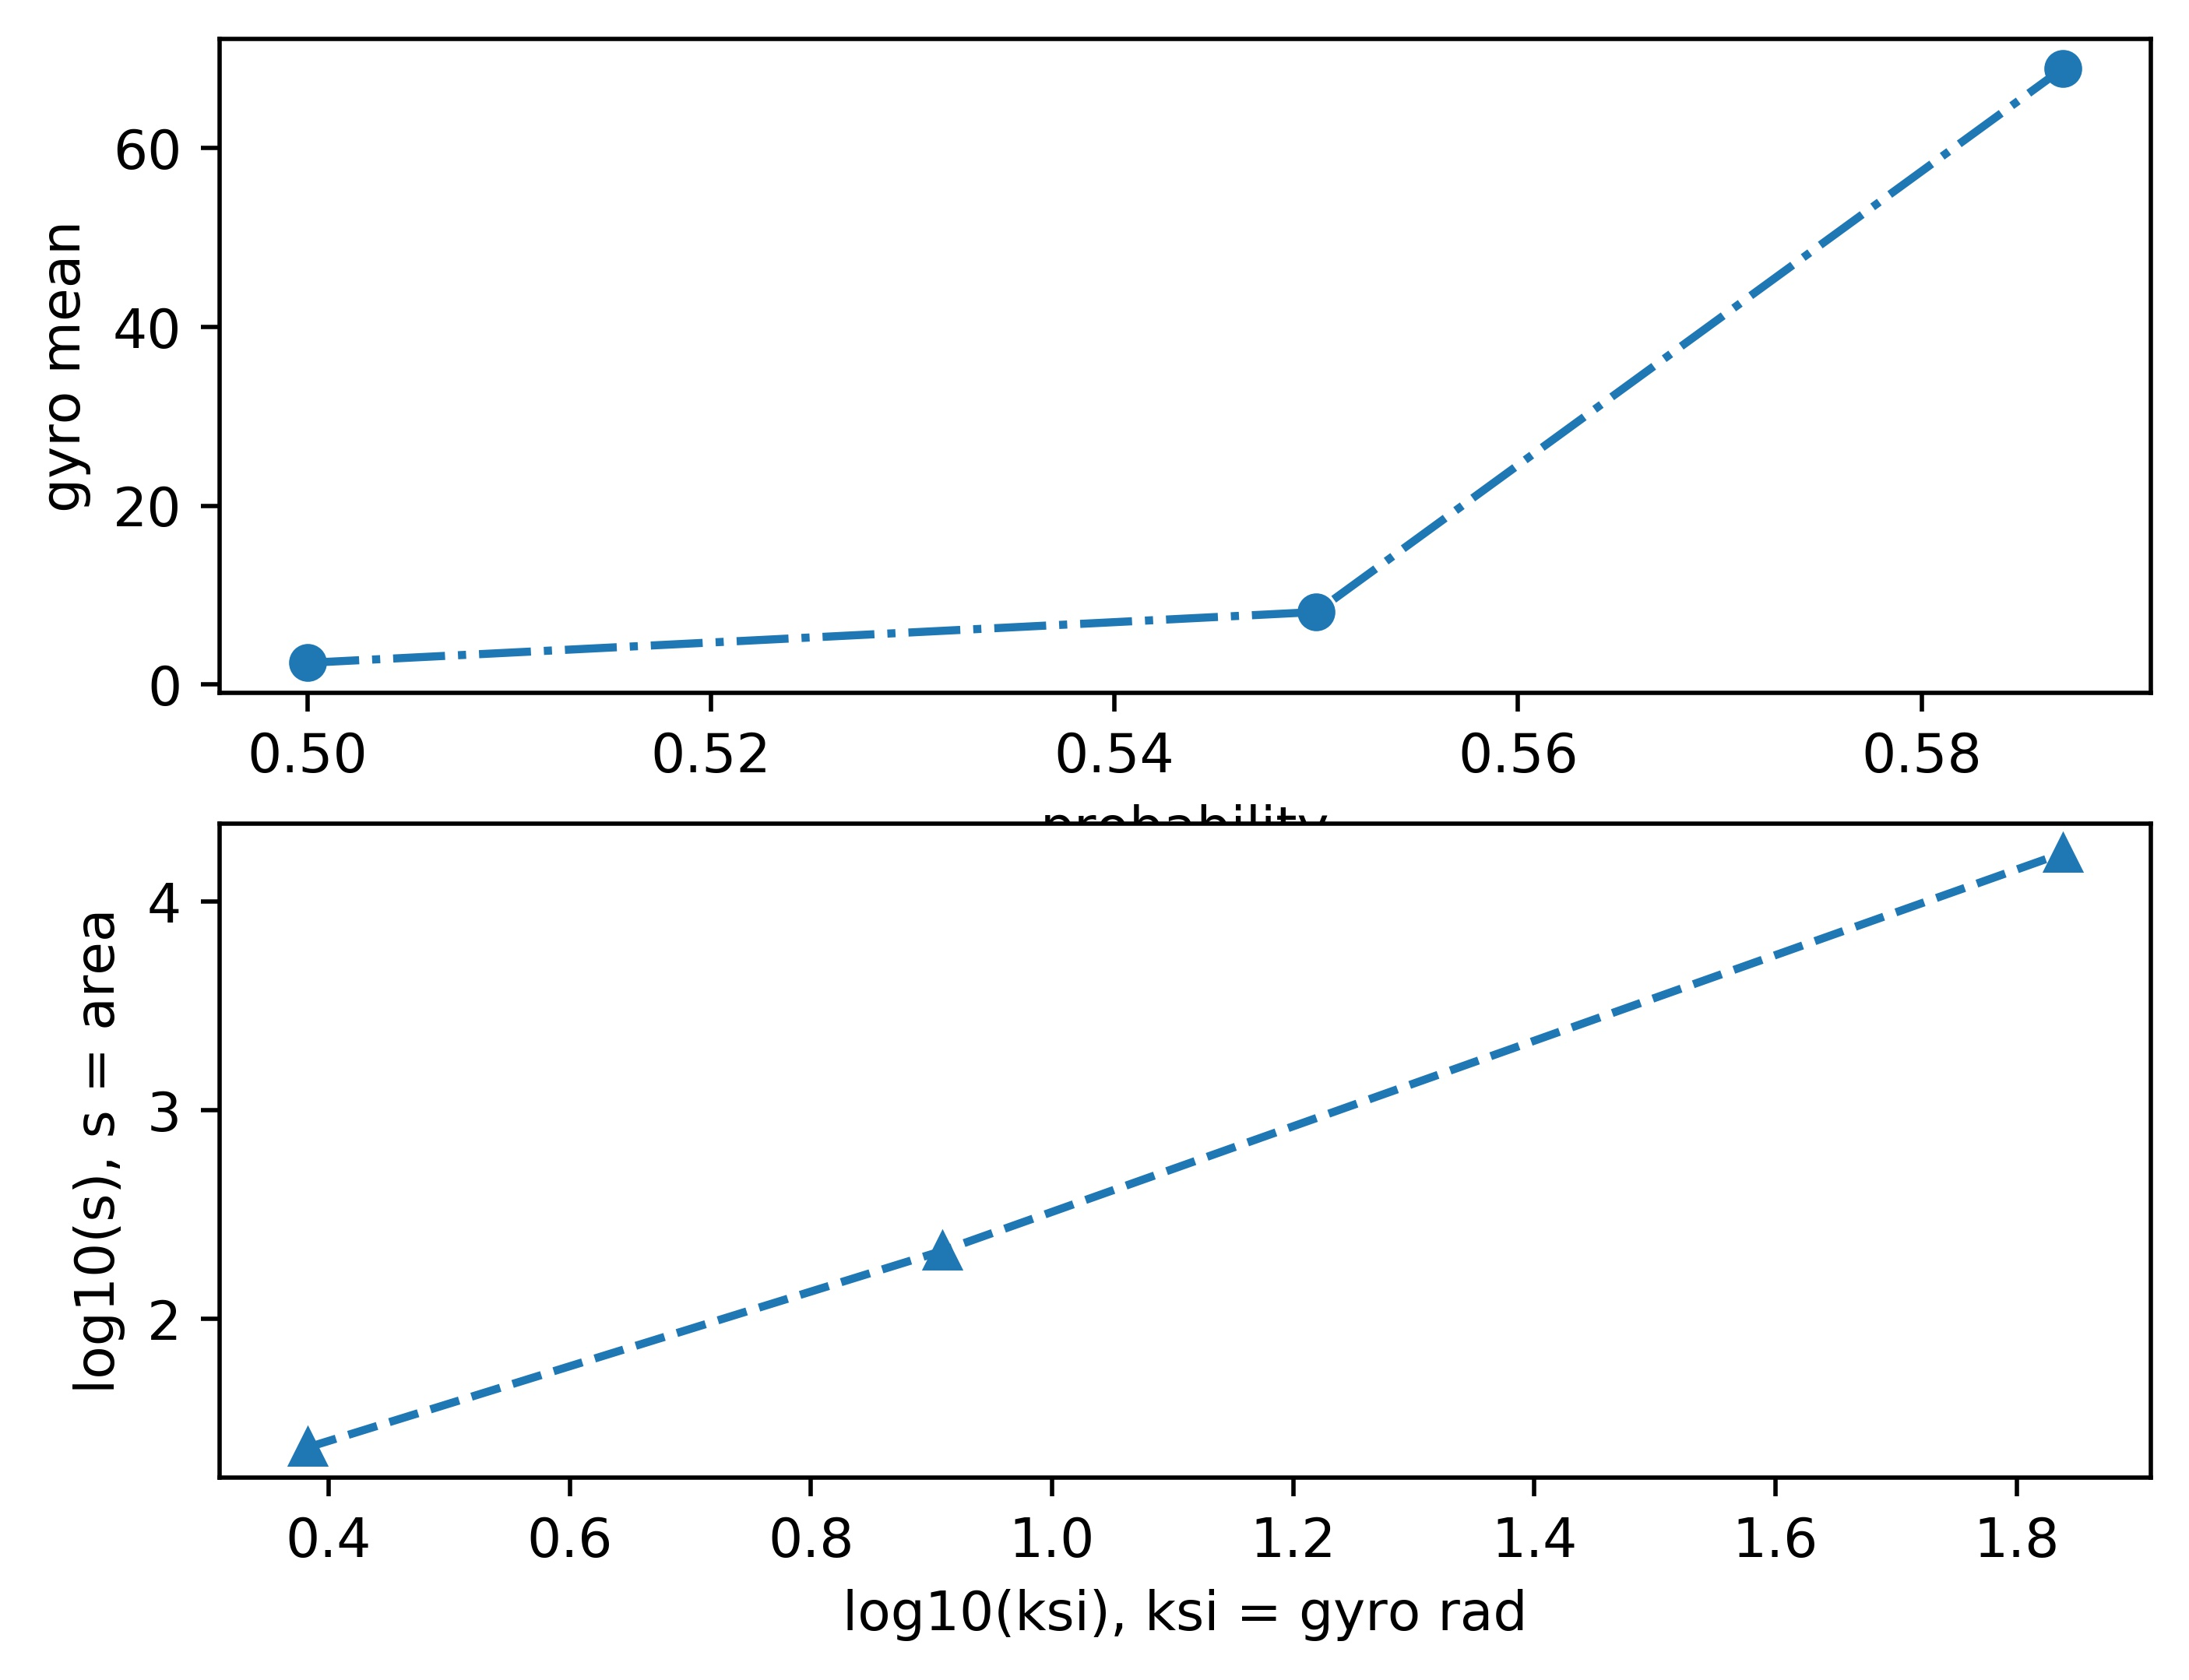
\includegraphics[width=0.9\linewidth]{../p7/area-gyro.jpg}
		\label{fig:area-gyro}
		\caption{I simulated the percolation 150 time for each probability and found reported the mean. Here
		in the top plot you see \emph{gyro radius} vs. \emph{probability}
		and \emph{log of area} vs. \emph{log of gyro radius} in the bottom plot.}
	\end{figure}
\end{document}